In high information and cognitive load tasks such as real-time monitoring of network security, social media monitoring, or urban traffic congestion, it is common to have large-scale visual interfaces to display current system status, alerts, and events~\cite{Landesberger2011,Liu2014,Sun2013}. However, the massive volume of available information prevents the simultaneous presentation of all information relevant to each alert or event~\cite{Liu2014}. Thus, adaptive user interfaces (AUIs) are necessary to filter information to provide localized and relevant context for each alert or event.  
Such AUIs allow the user to efficiently investigate the cause and implications of the alert or event, to identify critical properties of all the elements involved, and to initiate appropriate corrective actions in a timely manner.

In this work, we argue that this information-filtering task is central to a variety of AUIs.  Furthermore, we argue that the filtering task shares many common properties of a standard Information Retrieval (IR) setting as summarized in Table \ref{tbl:Comparaison2IR}.  Clearly there are important differences between ranking documents in web search and filter selection for AUIs, especially in the way that documents in the AUI can only be selected for a result set through filter settings.
However there is also substantial overlap and formal connection with many aspects of IR thus providing   
%especially in the indirect selection of AUI results through filter %settings. Hence this unexplored field 
%provides new possibilities for cross-pollination 
new opportunities and challenges of research in this novel IR setting for AUIs.



%The key difference is that while information retrieval is ubiquitous in the lives of most humans in the form of web search, it has gone virtually unrecognize as an appropriate model for the filtering problem in AUIs \textcolor{red}{[REFERENCE IS NEEDED]}. 
%Instead, machine learning methods have been widely used to address this problem.

\begin{figure}[t]
\begin{centering}
\subfigure[Global display showing anomalies.]{\includegraphics[width=4.25cm]{imgs/twitter_example}\label{Fig:GlobalDisplay}}\subfigure[Filtered and focused display.]{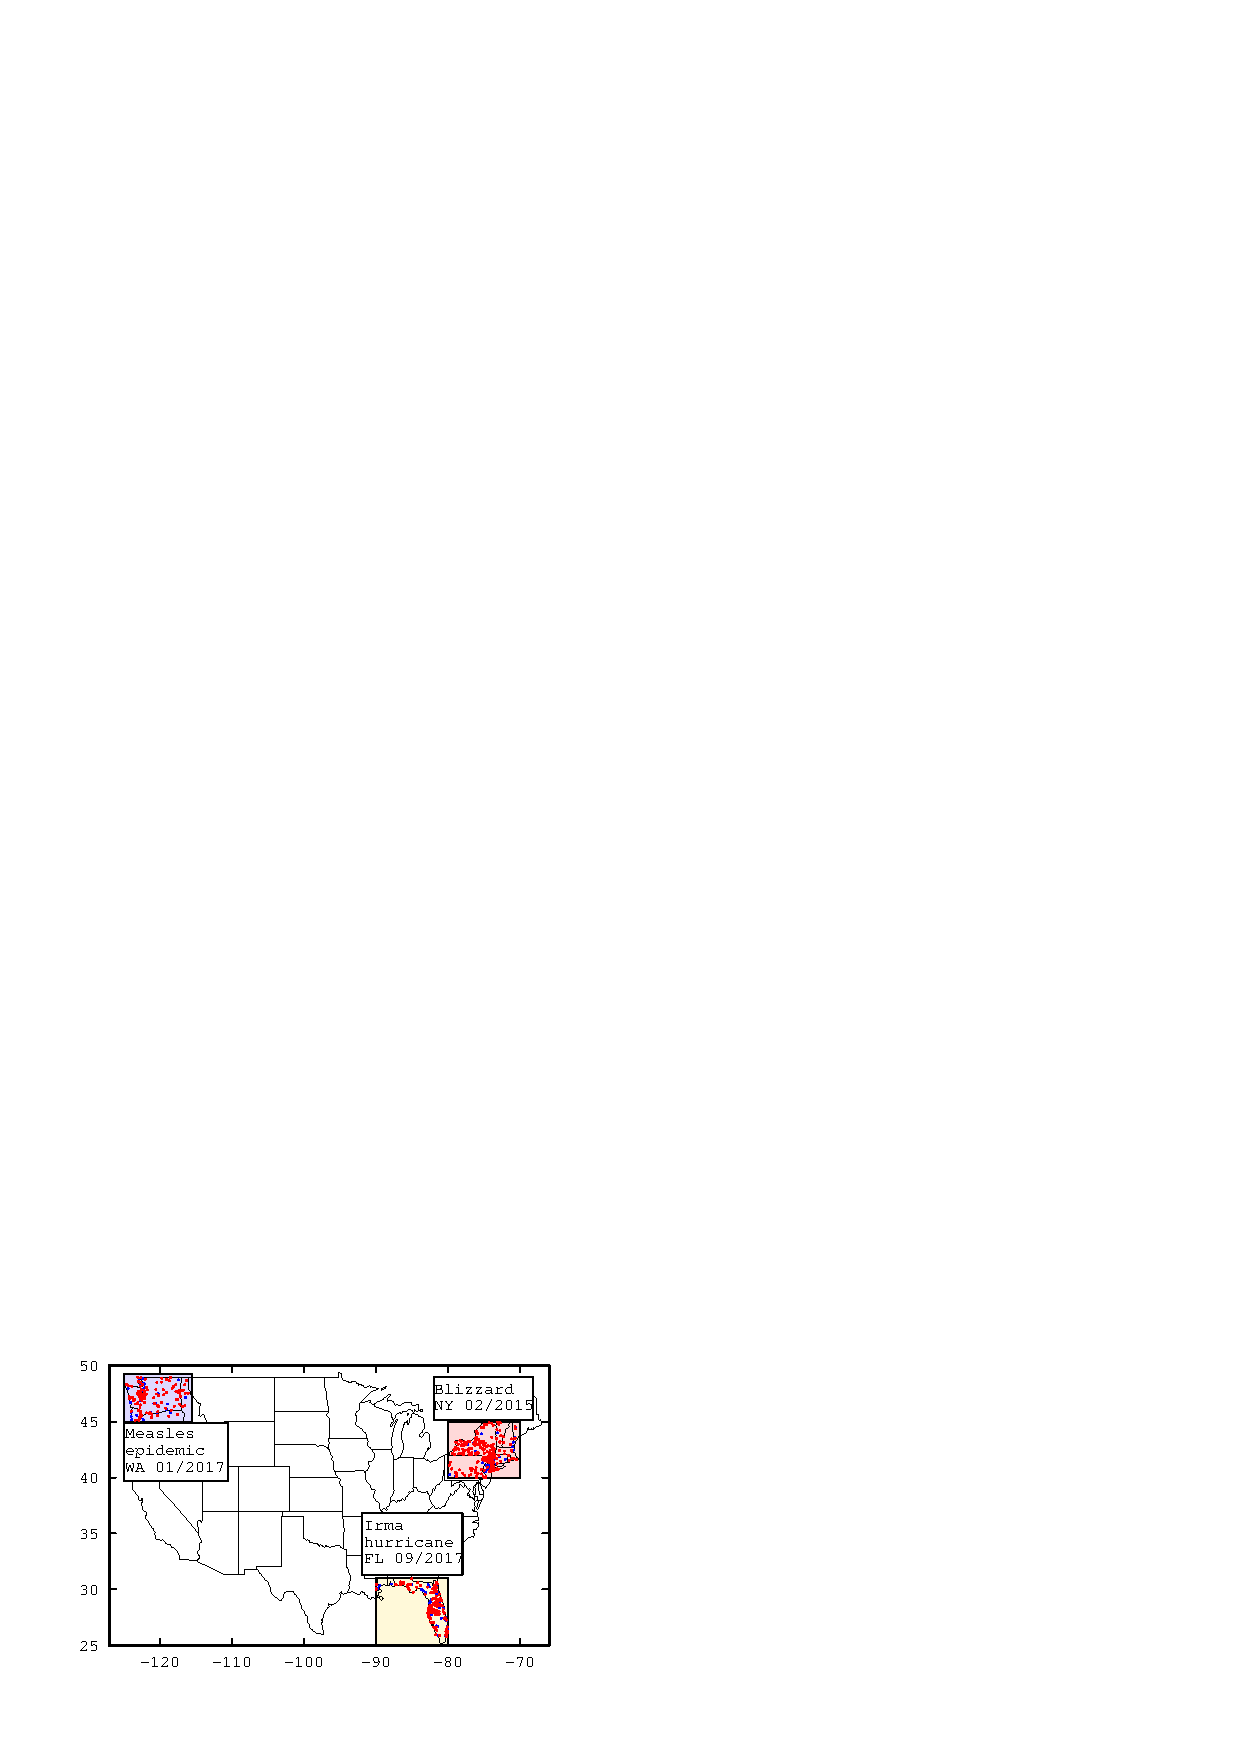
\includegraphics[width=4.25cm]{imgs/twitter_example_filter}\label{Fig:FilteredDisplay}} 
\par\end{centering}
\caption{(a) An unfiltered user interface with geolocated tweets appearing more red according to their probability of classification as natural disaster.  (b) A filtered version of the interface showing three filtered subsets of data identified to have high coverage of relevant content: a bounding box near New York state limited to data in Feb 2015 and having keyword ``Blizzard'' and other time and keyword restricted bounding boxes centered on Florida and Washington state.  An IR perspective on which objective to evaluate and how to choose these filters and filter settings to optimize surrogates of this objective is the focus of this paper.}
\label{Fig:UseCase}
\end{figure}

\begin{table*}[t]
\caption{Comparison between conventional Web Search and Filtering for AUIs.}
\label{tbl:Comparaison2IR}
\centering{}%
\begin{tabular}{|c|>{\centering}p{6cm}|>{\centering}p{6cm}|}
\hline 
 & \textbf{Web Search} & \textbf{Filtering for AUIs}\tabularnewline
\hline 
\hline 
\textbf{Information Need} & Realized by query  & Selection of an event or alert\tabularnewline
\hline 
\textbf{Form of Results} & Ranked list of documents & Filter settings (bounding box in visual display, time ranges, property
filters) that select a subset of information elements to display\tabularnewline
\hline 
\textbf{Relevance Scoring} & Comparison of query and document content (and other relevant information)
to generate a relevance score, e.g., via TF-IDF or BM25 & Third party application-specific tool (e.g., a machine learning approach)
that predicts the probability that each information element is relevant
to the selected alert\tabularnewline
\hline 
\textbf{Test Data for Benchmarking} & A set of queries; human-labeled judgments of document relevance to
each query for a test corpus (i.e., ground truth relevance) & A set of alerts or events; human-labeled judgments of information element relevance
to a selected alert (i.e., ground truth relevance)\tabularnewline
\hline 
\textbf{Evaluation} & Ranking metrics (P@k, AP, etc.) over documents given ground truth
relevance  & Boolean metrics (e.g., F1-score) and Ranking metrics (P@k, AP, etc.)
over information elements selected by the filter given ground truth
relevance \tabularnewline
\hline 
\end{tabular}
\end{table*}


To make the task of AUI filtering more concrete and to link it clearly
to information retrieval, let's introduce an example filtering
scenario for AUIs. 
Consider the case of monitoring events that are discussed on Twitter for the purpose of identifying natural disasters. Typically, as shown in Figure \ref{Fig:GlobalDisplay}, there would be some visual display of all raw information in the network along with relevant Tweets on diverse natural disasters (red nodes in Figure \ref{Fig:GlobalDisplay}). We denote all displayed content (in this case individual tweets)
%(such as user IP address, Tweet content, Tweet time, geographical coordinates, recent activity details) 
as an information element that could
be optionally shown or not.  Displaying all information elements simultaneously
would result in a saturated and an unreadable display for any reasonably sized 
 problem. To ease the investigation task, users could restrict the information displayed
through a variety of filter settings to get a clear overview of individual events as shown in Figure \ref{Fig:FilteredDisplay} \textendash{} by panning and
zooming in the graph display, by restricting upper and lower bounds
on a time filter, and/or by selecting properties (e.g., in a drop-down
selection or fielded keyword search in fields such as Tweet content). 
%\textcolor{red}{Such filter settings are expected to help a monitoring agent to efficiently investigate the cause and implications of the triggered alarm, to identify common properties of the elements involved in that alert, and to initiate appropriate corrective actions in a timely manner.}





While the user would typically find it hard to manually set these
filters to optimally reveal information about an anomaly they are
currently investigating, an AUI that is aware of the alert of interest
to the user and aware of the probability that each information element
is relevant to the alert could automatically suggest filter settings
that might display the relevant information element set with the least
amount of irrelevant clutter. Thus, the user could use these filter settings to carry out his investigation by identifying common properties of the elements involved in the alert, find the origin of the deficiency, and eventually, take a set of actions to address the problem.
We assume the prediction of information element relevance to an alert
to be provided by a third-party since this prediction is highly specific
to each particular application setting and not the focus of this work (see Related Work in Section 6 for further discussion). 
%In this work, we intend to
%focus on the broader problem of AUI filtering in a range of visual
%display applications assuming this relevance predictor is given. However,
%in addition to scoring information elements of direct causal interest
%to the alert, it is likely that the AUI will also contain other related material requiring
%the concurrent display of information.  For example, such a material could be messages exchanged, the time at which these messages were exchanged, etc.
%For example, such a rule could
%be \textquotedblleft if a connection is shown, the IP addresses of
%the two connected machines must also be shown\textquotedblright ,
%which would trigger additional (soft) constraints for the filter optimization.

Since \textquotedblleft retrieved\textquotedblright{} information
elements are not individually selected, but rather chosen through
a filter setting (that the user can further modify), the problem is clearly 
an optimization problem of how to restrict filter settings to show
the user the most relevant information to the alert or event they have to investigate.
While this diverges from the standard information retrieval setting
where ranked documents are chosen individually \cite{Baeza-Yates2010}, these additional constraints
do not change the overall information retrieval objective to select
relevant information given the user\textquoteright s information need. 
%Furthermore, standard information retrieval evaluation benchmarking
%methodology (e.g., the Cranfield paradigm) and metrics such as precision@k
%or average precision are also relevant here (assuming that visual
%saliency can serve as a surrogate method for achieving a visual rank
%ordering of selected information elements).  Unlike information retrieval
%where Boolean metrics such as F-Score are not often used since ranked
%lists are usually limited to the top-10, graphical displays can present
%substantially more information of varying sizes that make precision-recall
%trade-off metrics like F-Score also relevant for evaluation.\textcolor{red}{ [THIS SENCTENCE IS UNCLEAR]}

%With the aim of assisting network monitoring agents in carrying out their daily tasks, we present in this paper a new visual search paradigm for AUIs. 
To the best of our knowledge, this work is the first to address the AUI problem as an information retrieval problem of optimizing filter settings for relevance coverage. The contributions of this paper are summarized as follows: 
 \begin{enumerate}
\item We propose a new theory of IR for adaptive visual user interfaces. 
\item We propose new expected metrics for optimization based on conventional IR metrics, i.e., precision, recall, and F1-Score.
We argue that F1-Score and hence expected F1-Score is a good metric for this domain.
\item We propose new filter setting search algorithms based on greedy strategies and optimal solutions. These algorithms are based on the optimization of new proposed metrics.
%\item  We propose new MILP-based search method, which can also used about justification of new search algorithm.
\item We present a thorough evaluation on three different datasets to show that the greedy algorithms we propose are a good approximation of the optimal method, and perform well in the presence of noise (i.e., corruption of the ground truth labels).
%can even perform better with a noisy classifier \textendash{} up to 42\% improvement for a classifier with an accuracy of 60\%. On the other hand, 
We experimentally demonstrate that the expected F1-Score metric is a good surrogate of F1-Score.
%specifically with a highly accurate classifier \textendash{} for a classifier with 90\% accuracy, the RMSE is roughly 0.0111).
\end{enumerate}

%The rest of the paper is organized as follows: in Section \ref{sec:Framework},  presents the concepts and  the nation used throughout this paper;  Section \ref{sec:Algorithms} presents the new search algorithms of filter settings for AUIs; Sections \ref{sec:setup} and \ref{sec:Evaluation}  describe the evaluation setup and results respectively;  Section \ref{sec:RelatedWork}  discusses the related work; and Section \ref{sec:Conclusions} concludes with key observations and future research directions.



